\documentclass[xcolor=table,aspectratio=169]{beamer}
\errorcontextlines 10000
%\usepackage{polyglossia}
%\setmainlanguage[latesthyphen=true,spelling=new]{german}
%\usepackage[ngerman]{babel}

\hypersetup{pdfencoding=auto}

% ...and rename this to "Folie"
\newcommand{\slidenomenclature}{Page}

\usepackage[autostyle=tryonce]{csquotes}

\usepackage{tikz}
\usetikzlibrary{shapes.geometric}


\usepackage[export]{adjustbox}
\usepackage{tabularx}
\usepackage{colortbl}
%\setlength\extrarowheight{3pt}
\renewcommand{\arraystretch}{1.3}

\usepackage{amsmath}
\usepackage{bookmark}
\usepackage{booktabs}

\usepackage{pgfplots} % the package used to implement the graphs  
\usepgfplotslibrary{polar} % to determine the polar coordinates  
\usepgflibrary{shapes.geometric}  
\usetikzlibrary{calc}  
\pgfplotsset{width = 6.4cm, compat = newest} % it is the width of the graph. The lesser the width, the higher the graph will shrink.  
\usepackage{sansmath} % it is the package used in math. It provides the math font.  
\pgfplotsset{  
% pgfplotsset is used to define the parameters used further to draw a graphs  
  tick label style = { font=\tiny\sansmath\sffamily}, ,% it defines the font size of the label  
  label style = { font=\small\sansmath\sffamily}  
}  
\usepackage{physics}

\mode<presentation>
{
	\usetheme{ldv}
	% How to hide stuff (dimmed or really hidden)
%	\setbeamercovered{transparent}
	\setbeamercovered{invisible}
}

\title[SCCS Seminar | High Dimensional Methods | Adaptive Sparse Grids]{Adaptive Sparse Grids}
\subtitle{Seminar: High Dimensional Methods in Scientific Computing}
\subject{Presentation for my thesis}
\author{Muhammed K\"{u}r\c{s}at Yurt}

\date{\today}

\begin{document}

\frame{\titlepage}

\begin{frame}{Outline}
    \tableofcontents
\end{frame}

\section[]{Introduction}
\section{Introduction}

Ever increasing internet speed increased the data produced all around the world, that leads to boom in Machine Learning and Data Analytics fields.
Which are generally have many dimensional large data sets. As like all high dimensional problems, they are suffer from curse of dimensionality, i.e.\ they have an
exponential dependency on dimension. This is a barrier in numerical treatment of the high-dimensonal problems.
This exponential dependency makes harder to use classical mesh based approaches to solve this kind of problems. One could also use mesh-free methods like Monte-Carlo quadratures.

In order to overcome such a problem, the sparse grid method gains more and more popularity.
The sparse grid method is a general numerical discretization technique which is first introduced by  the Russian mathematician Smolyak in 1963~\cite{smolyak1963quadrature}.

Sparse grids offers a new way to reduce the required number of grid points by the order of magnitude \(O(2^{nd})\) to just only \(O(2^n n^{d-1})\) while preseving a similar error as using the full grid~\cite{Garcke2012}.
A comparision of storage requirement and error is listed in \cref{tab:comparisionfull}.
In order to achieve these bounds, the mixed second derivatives have to be bounded.

The sparse grid uses a hierarchical formulation as shown in \cref{fig:basiscomp} for one dimensional case.
It has an incremental and adaptive behaviour inherently. In order to extend to a general d-dimensional setting it expolits
tensor prodoct approach.

For the problems which are do not satisfy smoothness criteria or required further reduce in mesh size, one can use advantage of adaptivity.
The hierarchical basis is a direct indicator of areas where further refinement required.

\begin{figure}[hbpt]
    \centering
    \begin{subfigure}{0.45\textwidth}
        \includegraphics[width=\textwidth]{nodal_basis.pdf}
        \caption{Nodal Basis}
        \label{fig:nodalbasis}
    \end{subfigure}
    \begin{subfigure}{0.45\textwidth}
        \includegraphics[width=\textwidth]{hierarchical_basis.pdf}
        \caption{Hiearchical Basis}
        \label{fig:hierarchicalbasis}
    \end{subfigure}
    \caption{Comparision of piecewise linear basis functions.}
    \label{fig:basiscomp}
\end{figure}

\begin{table}[hbpt]
    \centering
    \caption{Comparision of Sparse and Full Grid Approaches.}
    \begin{tabular}{l c c}
        \multicolumn{1}{c}{} & Storage Requirement  & \multicolumn{1}{c}{L2 Norm of Interpolation Error} \\
        \toprule
        Full Grid            & \(O(2^{nd})\)        & \(O(2^{-2n})\)                                     \\
        \midrule
        Sparse Grid          & \(O(2^{n} n^{d-1})\) & \(O(2^{-2n} n^{d-1})\)                             \\
        \bottomrule
    \end{tabular}
    \label{tab:comparisionfull}
\end{table}

In this work we will use standard hat function given by \cref{eqn:basis}.

\begin{equation}
    \phi(x ) = \left\{
    \begin{array}{ll}
        1-|x| & \text{if } x \in [-1,1] , \\
        0     & \text{otherwise}          \\
    \end{array}
    \right.
    \label{eqn:basis}
\end{equation}

On a equidistant grid \(\Omega_l \) of level \( l\) on a unit interval \(\bar{\Omega} = [0,1]\). The mesh width is given by \(2^{-l} \). The grid points on a certain level is given bibliography

\begin{equation}
    x_{l,i} = i \cdot h_l, 0 \leq i \leq 2^l
\end{equation}

Using \cref{eqn:basis} a family of basis functions \(\phi_{l,i}(x)\) with a support of \([x_{l,i}-h_l,x_{l,i}+h_l]\), by dilation and translation one could get \cref{eqn:levelbasis}. This process gives all possible basis function in level \(l\) as shown in \cref{fig:nodalbasis}.

\begin{equation}
    \phi_{l,i}(x) = \phi \left(\frac{x-i\cdot h_l}{h_l}\right)
\end{equation}

\begin{equation}
    V_l = \text{span} \left\{ \phi_{l,i} : 1 \leq i \leq 2^l-1 \right\}
    \label{eqn:levelbasis}
\end{equation}

One need hierarchical ones in order to construct the sparse grid. The hierarchical increment spaces are given by \cref{eqn:hierarchicalincrementspace}.

\begin{equation}
    W_l = \text{span} \left\{ \phi_{l,i} : i \in I_l\right\}
    \label{eqn:hierarchicalincrementspace}
\end{equation}

where the index set is,

\begin{equation}
    I_l = \left\{ i \in \mathbb{N}: 1 \leq i \leq 2^l-1 , i \text{ odd} \right\}
\end{equation}

Using the resulting basis functions as input to the tensor product construction, one can obtain suitable piecewise d-linear basis function at each grid point \(x_{l,i}\)

\begin{equation}
    \phi_{l,i}(x) = \prod_{j=1}^d \phi_{l_j,i_j}(x_j)
\end{equation}

\section[]{A deeper look to Sparse Grids}

\begin{frame}{Sparse Grids}{Requirements for a sparse grid}
    \begin{itemize}[<+->]
        \item A scalar valued function \(f\) which maps some input parameter \(\vb{x}\) to a scalar value \(f(\vb{x})\).
        \item \(f\) is defined on a unit hyper-cube \([0,1]^d\). Any input \(x_i\) should be transformed to \([0,1]\) easily.
        \item \(f\) can be computable in any point in hyper-cube.
        \item It is assumed that the function is \emph{computatinally expensive}. So that we need to change \(f\) with another function which is \emph{cheaper} and approximate original function well.
    \end{itemize}
\end{frame}

\begin{frame}{Sparse Grids}{Hierachical Basis Functions}
    \begin{columns}
        \begin{column}{0.5\textwidth}
            Using a standard hat function as a basis function, we can construct a sparse grid.

            \begin{equation*}
                \phi(x ) = \left\{
                \begin{array}{ll}
                    1-|x| & \text{if } x \in [-1,1] , \\
                    0     & \text{otherwise}          \\
                \end{array}
                \right.
                \label{eqn:basis}
            \end{equation*}
            \begin{figure}
                \centering
                \includegraphics[width=\textwidth]{figures/nodal_basis.pdf}
                \caption{Nodal Basis Functions}
            \end{figure}
        \end{column}
        \begin{column}{0.5\textwidth}
            \begin{figure}
                \centering
                \includegraphics[width=\textwidth]{figures/hierarchical_basis.pdf}
                \caption{Hierarchical Basis Functions}
            \end{figure}
        \end{column}
    \end{columns}

\end{frame}

\begin{frame}{Sparse Grids}{Tensorial product and construction on d-dimensional space}
    \begin{figure}
        \centering
        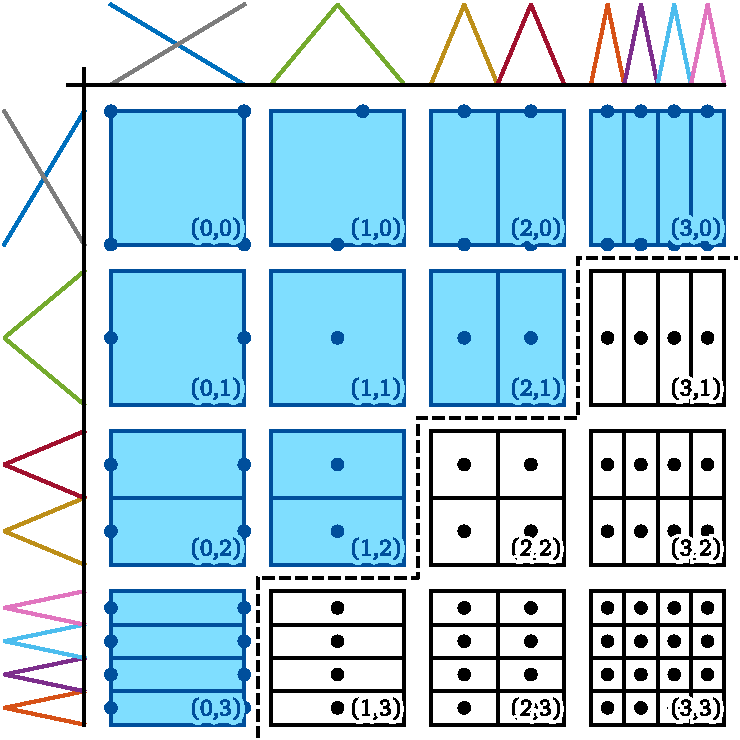
\includegraphics[width=\textwidth,height=0.6\textheight,keepaspectratio]{figures/sg_construction.pdf}
        \caption{Construction of the regular sparse grid of level in 2D, by \emph{Julian Valentin}}
    \end{figure}
\end{frame}


\section[]{Adaptivity on Sparse Grids}

\section{Adaptivity}

A regular sparse grid is constructed in a way that takes a cut in diagonal hyperplane, which means
it treats all the dimensions equally. However, there can be an importance difference between the dimensions,
i.e. one dimension might be more important than others. This can be solved by so called dimensional adaptivity.

The most straightforward approach for this type of refinement is adding some
new subspaces in the dimension which function changes rapidly. In order to add a new subspace
\(W_{\vec{l}}\) one should include all the backward neighbours in the current set of subspaces.
This refiment treads all the grid points in one dimension as a uniform way,and called as
dimensionally adaptive refinement. Leads more point in one dimension than other one.

\todok{May be add an example of dimensionally adaptive sparse grid to here.}

Morever, there are some cases exist, where dimensional adaptivity is not to be enough to solve problem.
For instance take a function that is mostly flat, have peaks at certain regions in the domain.
Franke's function is a good example for this~\cite{Franke1979}.

\begin{equation}
    \begin{aligned}
        f(\textbf{x}) & = \frac{3}{4} \exp \left( - \frac{(9x_1-2)^2}{4} - \frac{(9x_2-2)^2}{4} \right) \\
                      & + \frac{3}{4} \exp  \left( - \frac{(9x_1+1)}{49} - \frac{9x_2+1}{10}\right)     \\
                      & + \frac{1}{2} \exp \left( -\frac{(9x_1-7)^2}{4} - \frac{(9x_2-3)^2}{4} \right)  \\
                      & - \frac{1}{5} \exp \left( - (9x_1-4 )^2 -(9x_2-7)\right)
    \end{aligned}
\end{equation}

\begin{figure}
    \centering
    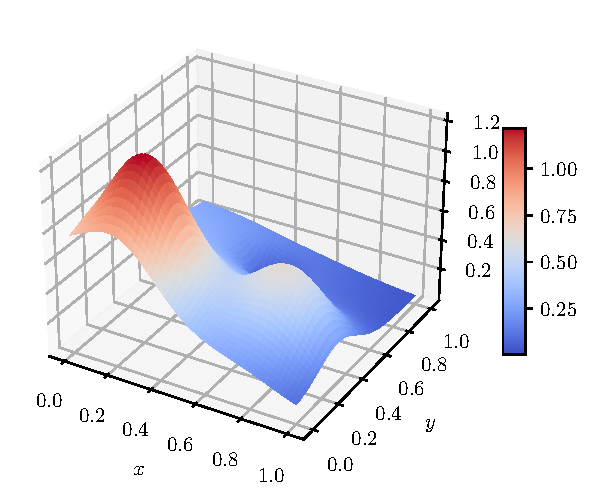
\includegraphics[width=0.4\textwidth]{figures/franke.pdf}
    \caption{Surface plot of Franke's Function.}
    \label{fig:franke}
\end{figure}

A dimensionally adaptive grid would also add more point to regions where the function is mostly flat.
A spatially adaptive grid would overcome this problem. Instead of adding whole incremental grids,
spatial adaption would only include a subset of those points near the region of interest and saves points.

The general approach for spatially adaptive grids is doing the refinement process iteratively.
One could start and initial coarse grid or if knows a grid which is tailored to problem. Using an iterative process
one could simply adds new points (neighboring grid point in the next higher level) to region of interest. To enable usage
of sparse grids algorithms there is also a consistency constraint exist, the grid should contain all the hierarchical
ancestors of all grid points. Figure~\ref{fig:spatialrefiment} shows how this process is done in two-dimensional regular sparse grid.

\begin{figure}
    \centering
    \missingfigure{Add refiment figure here.}
    \caption{Spatial refinement of a selected node in two dimension.}
    \label{fig:spatialrefiment}
\end{figure}

\section[]{Sparse Grid in Action: Interpolation}


\section{Examples}


\subsection{Spatial Adaptivity}




\begin{frame}
    \centering
    \LARGE{Thank you for your attention!}
\end{frame}
\end{document}
